\documentclass[12pt,a4paper,twoside,openright]{report}
\usepackage{algpseudocode}		% ambienti per la scrittura di algoritmi
\usepackage{algorithm}			% 

\usepackage{epsfig}						% figure eps
\usepackage{graphicx}					% figure qualsiasi
\usepackage{amsmath,amsfonts,amsthm}		% package di scrittura matematica
\usepackage{amssymb}
\usepackage{psfrag}
\usepackage{fancyhdr}
\usepackage{u

\end\documentclass{beamer}

% \usepackage{beamerthemesplit} // Activate for custom appearance

\title{Example Presentation Created with the Beamer Package}
\author{Till Tantau}
\date{\today}

\begin{document}

\frame{\titlepage}

\section[Outline]{}
\frame{\tableofcontents}

\section{Introduction}
\subsection{Overview of the Beamer Class}
\frame
{
  \frametitle{Features of the Beamer Class}

  \begin{itemize}
  \item<1-> Normal LaTeX class.
  \item<2-> Easy overlays.
  \item<3-> No external programs needed.      
  \end{itemize}
}2
\end{document}
\begin{figure}[htbp] %  figure placement: here, top, bottom, or page
   \centering
   \includegraphics[width=2in]{example.jpg} 
   \caption{example caption}
   \label{fig:example}
\end{figure}\documentclass[11pt, oneside]{article}   	% use "amsart" instead of "article" for AMSLaTeX format
\usepackage{geometry}                		% See geometry.pdf to learn the layout options. There are lots.
\geometry{letterpaper}                   		% ... or a4paper or a5paper or ... 
%\geometry{landscape}                		% Activate for for rotated page geometry
%\usepackage[parfill]{parskip}    		% Activate to begin paragraphs with an empty line rather than an indent
\usepackage{graphicx}				% Use pdf, png, jpg, or eps§ with pdflatex; use eps in DVI mode
								% TeX will automatically convert eps --> pdf in pdflatex		
\usepackage{amssymb}

\title{Brief Article}
\author{The Author}
%\date{}							% Activate to display a given date or no date

\begin{document}
\maketitle
%\section{}
%\subsection{}



\end{document}  % XeLaTeX can use any Mac OS X font. See the setromanfont command below.
% Input to XeLaTeX is full Unicode, so Unicode characters can be typed directly into the source.

% The next lines tell TeXShop to typeset with xelatex, and to open and save the source with Unicode encoding.

%!TEX TS-program = xelatex
%!TEX encoding = UTF-8 Unicode

\documentclass[12pt]{article}
\usepackage{geometry}                % See geometry.pdf to learn the layout options. There are lots.
\geometry{letterpaper}                   % ... or a4paper or a5paper or ... 
%\geometry{landscape}                % Activate for for rotated page geometry
%\usepackage[parfill]{parskip}    % Activate to begin paragraphs with an empty line rather than an indent
\usepackage{graphicx}
\usepackage{amssymb}

% Will Robertson's fontspec.sty can be used to simplify font choices.
% To experiment, open /Applications/Font Book to examine the fonts provided on Mac OS X,
% and change "Hoefler Text" to any of these choices.

\usepackage{fontspec,xltxtra,xunicode}
\defaultfontfeatures{Mapping=tex-text}
\setromanfont[Mapping=tex-text]{Hoefler Text}
\setsansfont[Scale=MatchLowercase,Mapping=tex-text]{Gill Sans}
\setmonofont[Scale=MatchLowercase]{Andale Mono}

\title{Brief Article}
\author{The Author}
%\date{}                                           % Activate to display a given date or no date

\begin{document}
\maketitle

% For many users, the previous commands will be enough.
% If you want to directly input Unicode, add an Input Menu or Keyboard to the menu bar 
% using the International Panel in System Preferences.
% Unicode must be typeset using a font containing the appropriate characters.
% Remove the comment signs below for examples.

% \newfontfamily{\A}{Geeza Pro}
% \newfontfamily{\H}[Scale=0.9]{Lucida Grande}
% \newfontfamily{\J}[Scale=0.85]{Osaka}

% Here are some multilingual Unicode fonts: this is Arabic text: {\A ?????? ?????}, this is Hebrew: {\H ????}, 
% and here's some Japanese: {\J ???}.



\end{document}  

\endrl}
\usepackage{array}
\usepackage{subfigure}
\usepackage{lscape}
\usepackage{colortbl}
\usepackage{alltt}
\usepackage{tabularx}
\usepackage[english]{babel}
\usepackage[nottoc]{tocbibind}
\sloppy
\raggedbottom

\linespread{1.3}
\renewcommand{\baselinestretch}{1.3}

\makeatletter
\def\cleardoublepage{\clearpage\if@twoside \ifodd\c@page\else
\hbox{}
\vspace*{\fill}
\begin{center}
%This page intentionally contains only this sentence.
\end{center}
\vspace{\fill}
\thispagestyle{empty}
\newpage
\if@twocolumn\hbox{}\newpage\fi\fi\fi}
\makeatother

%\newcites{wb}{Web References}

%------------------------------------------------------
% Impostazioni per il controllo sillabazione vedove/orfane ect..
%
% \looseness=1 o \looseness=-1 prima di un paragrafo per
% allungarlo o accorciarlo di una riga
%------------------------------------------------------

\lefthyphenmin=4
\righthyphenmin=4
\tolerance=1000
\hyphenpenalty=100
\emergencystretch=1 cm

\widowpenalty=5000
\clubpenalty=2500

%--------------------------------------------------------
% impostazioni per la dimensione delle pagine
%--------------------------------------------------------
\renewcommand{\headrulewidth}{0.5pt}
\hoffset=-15mm
%\topmargin=0mm
\headheight=15pt
\textwidth=140mm
\headsep=5mm
\voffset=-5mm
%\hsize=13cm
%\textwidth=164mm
\textheight=230mm
\evensidemargin=25mm
\oddsidemargin=25mm
%\marginparwidth=0mm

\renewcommand{\abovecaptionskip}{0pt}
\renewcommand{\belowcaptionskip}{0pt}

%--------------------------------------------------------------
%impostazione headers
%--------------------------------------------------------------
\pagestyle{fancy}
%\addtolength{\headwidth}{\marginparsep}
%\addtolength{\headwidth}{\marginparwidth}
\renewcommand{\chaptermark}[1]{\markboth{#1}{}}
\renewcommand{\sectionmark}[1]{\markright{\thesection\ #1}}
\fancyhf{}
\fancyfoot[LE,RO]{\bfseries\thepage}
\fancyhead[RO]{\bfseries\rightmark}
\fancyhead[LE]{\bfseries\leftmark}
\fancypagestyle{plain}{%
\fancyhead{} % get rid of headers
\fancyfoot{}
\renewcommand{\headrulewidth}{0pt} % and the line
}

\newenvironment{myverse}
{\small}
{}

\newenvironment{myabstract}{%
  \begin{center}%
    \null\vfil
    \bfseries \abstractname
  \end{center}}%
{\par\vfil\null}

%------------------------------------
\newcommand{\name}{$\mathcal{H}$eaven } 
\newcommand{\namens}{$\mathcal{H}$eaven} 
%------------------------------------
\begin{document}

\pagenumbering{roman}
\setcounter{page}{1}
\pagestyle{empty}

%--------------------------------------------------------------------------------
% include title page
%--------------------------------------------------------------------------------
%\linespread{1}
\begin{titlepage}
\vspace*{-2.5cm}
\bfseries
\begin{center}
  \LARGE
  Politecnico di Milano\\
  \Large
  School of Industrial and Information Engineering\\

\psfig{file=images/logopm,width=4cm}

\begin{large}
Department of Electronic, Informatics and Bioengineering\\
Engineering of Computer Systems\\
\end{large}

\vspace{1.0cm}
\begin{Large}
\namens: Supporting Systematic Comparative Research of RDF Stream Processing Engines
\end{Large}  
\end{center}
\vspace*{4.5cm}
\large
\begin{flushleft}
\hspace{-2cm}  Advisor: Emanuele DELLA VALLE\\
\hspace{-2cm}  Co-Advisor: Daniele DELL'AGLIO\\
\end{flushleft}
\vspace*{1.5cm}

\hspace{1.5cm}
\parbox{14cm}{
    \begin{tabular}{lll}
        Master thesis by: & Riccardo TOMMASINI    & matr. 799120\\
    \end{tabular}
}

\vspace*{1.4cm}
\begin{center}

  Academic Year 2013-2014



\end{center}
\end{titlepage}
\cleardoublepage

%--------------------------------------------------------------------------------
% dedica
%--------------------------------------------------------------------------------
\thispagestyle{empty}

\begin{flushright}
\large\textit{To Aldo\\ }
%\large\textit{I miss you\dots\\}
\large\textit{and to my family,\\ }
\large\textit{thanks for all your support (and the fish)\dots\\}


\end{flushright}

%\null\vfil

\cleardoublepage

%--------------------------------------------------------------------------------
% ringraziamenti
%--------------------------------------------------------------------------------
\thispagestyle{empty}

\chapter*{Acknowledgements}

\begin{flushleft}
Milano, 1 Aprile 2015
\end{flushleft}
Ringrazio il Professor Emanuele Della Valle, che ha reso la tesi un percorso incredibilmente formativo. \`E stato un lavoro impegnativo, ma sempre stimolante e divertente. Grazie per l'opportunit\`a, il tempo dedicatomi e l'infinita quantit\`a di suggerimenti ricevuti. Sono grato anche a Daniele Dell'Aglio, per la sua guida e l'aiuto tecnico e per aver reso stimolante ogni discussione. Un sentito ringraziamento anche a Marco Balduini, per il suo prezioso contributo, in un momento, per lui, sicuramente molto difficile.

Ringrazio la mia famiglia, per avermi sostenuto nelle piccole difficolt\`a quotidiane, che da solo non avrei mai potuto superare, e per avermi insegnato che vale sempre la pena impegnarsi al massimo.

Ringrazio gli amici della MTF, per non avermi permesso di abbandonarli del tutto e per aver condiviso momenti unici e di incredibile sincerit\`a.

Ringrazio Teto. Cinque anni fa abbiamo iniziato insieme questa corsa e, come uno di famiglia, ci sei stato fino alla fine.

Ringrazio Francesco, per tutte le discussioni assurde che abbiamo fatto, i consigli onesti e per essere un vero amico da pi\`u di dieci anni.

Ringrazio Fabiana, per essere stata una guida spirituale, per avermi motivato e per aver sciolto nodi che stanno nella mia testa e nel cuore, non solo nei muscoli. Ringrazio anche Alberto, perch\`e lavora sempre dietro le quinte.

Ringrazio i Bomber, Fabio e Lorenzo. Per avermi mostrato come ci si diverte lavorando; per avermi dimostrato che chi punta in alto arriva in alto e soprattutto per avermi insegnato che "Nobody Works Like Us". Che dire ragazzi, se non "\textit{we were stuck in a blender, and now we are saving lives. WHAT?}"

\begin{flushright}
\emph{Riccardo}
\end{flushright}

\cleardoublepage
\thispagestyle{empty}

\pagestyle{fancy}
\renewcommand{\contentsname}{Table of Contents}%

%--------------------------------------------------------------------------------
% include the abstract in italian
%--------------------------------------------------------------------------------
\chapter*{Estratto}
Lo Stream Reasoning \`e  il settore di ricerca che ha dimostrato la possiblit\`a di applicare procedure di reasoning su flussi informativi in rapido cambiamento. Un RDF Stream Processing (RSP) Engine \`e  un sistema in grado di processare a livello semantico questi flussi, quando sono codificati secondo lo standard RDF. Il numero di RSP Engine implementati \`e  in crescita e di conseguenza la comunit\`a scientifica sta formalizzando i metodi e gli strumenti che hanno consentito lo sviluppo di queste soluzioni.

Diversi settori di ricerca nell'ambito della Computer Science, hanno mostrato interesse per una maggiore comprensione della natura del proprio lavoro. Sono stati fatti diversi studi che hanno analizzato i frutti della ricerca in questi settori~\cite{Tichy:1995:EEC:209090.209093, Wainer:2009:EEC:1518331.1518552}. Questi hanno dimostrato anzitutto la natura ingegneristica di molte pubblicazioni nell'ambito della Computer Science, ma anche una discreta mancanza di valutazioni empiriche delle soluzioni implementate. Questa \`e  una differenza evidente con le altre aree di ricerca legate al mondo dell'ingegneria, che si focalizzano su questo tipo di analisi.

Solitamente, nei settori informatici in cui la valutazione empirica \`e tralasciata, i sistemi proposti hanno una natura complessa e sfaccettata che \`e difficile da valutare. Tuttavia \`e  possibile, con gli strumenti adatti, studiare anche casi complessi. Questo accade per le scienze sociali o l'economia, i cui soggetti d'indagine non sono di certo facilmente modellabili. In questi settori viene comunemente usato un approccio comparativo sistematico, che semplifica il problema di affrontare soggetti complessi, senza tralasciare gli aspetti che li rendono rilevanti. Questo approccio diventa applicabile solo in un contesto sperimentale appropriato, che garantisce propriet\`a come riproducibilit\`a, ripetibilit\`a e comparabilit\`a.

La comunit\`a dello Stream Reasoning ha colto la necessit\`a di fornire strumenti per valutare correttamente gli RSP Engine,  comprenderne il comportamento e quantificarne il valore comparando le prestazioni in casi d'uso reali. Qualche passo in questa direzione \`e  stato gi\`a fatto. Lavori recenti~\cite{Zhang2012, LePhuoc2012c, DBLP:conf/semweb/DellAglioCBCV13} hanno fornito framework di benchmarking per RSP Engine, mentre altri hanno posto le basi di queste valutazioni~\cite{DBLP:conf/esws/ScharrenbachUMVB13}, mostrando quali erano le mancanze di tali framework.

Le soluzioni proposte si sono dimostrate limitate, e la valutazione empirica di RSP Engine \`e  solo all'inizio. Quello che ancora manca \`e  una infrastruttura che permetta la comparazione sistematica di RSP Engine, all'interno di un contesto sperimentale che goda delle proprit\`a sopracitate. Per affrontare il problema, in questa tesi, abbiamo preso dall'ingegneria aerospaziale l'idea di un banco di prova, uno strumento di valutatione e sviluppo per motori.

Un banco di prova permette di progettare esperimenti ed eseguirli su qualsiasi motore, raccogliendo i dati per una successiva valutazione delle prestazioni. 
La nostra domanda di ricerca quindi \`e : "Un banco di lavoro per RSP Engine \`e  la soluzione che permetta la ricerca comparativa e sistematica nell'ambito dello Stream Reasoning?"

In questa tesi proponiamo \namens, un framework open source per la ricerca comparativa e sistematica nell'ambito dello Stream Reasoning. Il framework si compone di un Banco di Lavoro, l'equivalente di quanto abbiamo visto nell'ingegneria aerospaziale ma per RSP Engine. Include quattro implementazioni naive di RSP Engine, dette Baselines. Questi sistemi semplificati permettono di iniziare la ricerca comparativa. Infine \name contiene l'Analyser, un insieme di metodi di indagine e strumenti di supporto, organizzati gerarchicamente ed atti ad analizzare e comparare i dati raccolti attraverso l'esecuzione di esperimenti su RSP Engine tramite il banco di lavoro.


%--------------------------------------------------------------------------------
% include the abstract in english
%--------------------------------------------------------------------------------
\chapter*{Abstract}
Stream Reasoning research field is grown enough to prove that reasoning upon rapidly changing information is possible. The number of working proposals for RSP Engines, systems capable to handle at semantic level RDF-encoded information flows, is increasing. Now the Stream Reasoning community is working on the standardisation of the methods and tools that supported the development of those solutions. Moreover, it is mandatory to provide an evaluation of RSP Engines, which allows to understand how these systems perform in real uses cases. 
Recent works in the filed \cite{Zhang2012, LePhuoc2012c, DBLP:conf/semweb/DellAglioCBCV13} has pursued this goal, providing many Benchmarking frameworks for evaluating RSP Engines. Further analysis of RSP Engines have point out the challenges involved by the Stream Reasoning research. They have posed the basis for a proper evaluation of such a system, describing in detail where these works have failed and where the can be improved \cite{DBLP:conf/esws/ScharrenbachUMVB13}. 

In parallel, many  Computer Science (CS) research fields have tried to understand the nature their own research. The related studies \cite{Tichy:1995:EEC:209090.209093, Wainer:2009:EEC:1518331.1518552} have shown the affinity of many CS research fields to an Engineering epistemology. But they have also evinced and criticised the concrete differences with other engineering research areas, which focus on evaluation and not only on the design and development of the proposed systems. The lacks of an empirical approach can be ascribed to the complex nature of the software systems. However, it is possible to face complex case studies which are not be easily modelled. Social science and economy researchers have found methods to deal with them.

The Stream Reasoning research suffers from the same lack. The limitations of the existing benchmarking proposals have proved that the empirical evaluation of RSP Engine systems is just at the beginning, and what is missing in an infrastructure which allows to compare the evaluations of RSP Engines. We borrow from the aerospace engineering the idea of an engine test stand. It is an automatic facility to design experiments and to execute them on any engine, under controlled conditions. Experiment properties like reproducibility, repeatability and comparability represent the pillars upon which we can start the empirical evaluation of RSP Engines. Thus, we formulate the following research question: "\textit{Can an engine test stand, together with queries, datasets and methods, support SCRA for Stream Reasoning?}"

In this thesis we propose \namens, an open source framework that enable the  Systematic Comparative Approach to the research of RSP Engine. It consists first in and engine Test Stand, the analogous of the aerospace engineering facility in the Stream Reasoning context. \name contains also four Baselines, which are naive implementations of RSP Engines. They represent  simple terms of comparison that can start the comparative research. Finally, \name enable the comparative analysis of RSP Engines at different levels trough the Analyser: a set of methods and tools, organised into an investigation stack.


%--------------------------------------------------------------------------------
% talbe of contents
%--------------------------------------------------------------------------------
\tableofcontents
\cleardoublepage

\pagenumbering{arabic}

\setcounter{page}{1}


%--------------------------------------------------------------------------------
% introduction
%--------------------------------------------------------------------------------
\chapter{Introduction}
\label{chap:introduction}
Stream Reasoning (SR) is a multidisciplinary research field that supports methods and tools which allow to answer complex queries like "What are the top five trend topics, under discussion on Twitter, and who is driving the discussions in Dayton?" or "How a certain event in Milan influences the user activity on Instagram?". The application domains of SR are not limited to social media analytics only. Semantic interpretation of sensor data, traffic monitoring and stream data integration are all possible use cases for SR \cite{DBLP:journals/expert/ValleCHF09}.

Stream Reasoning research has the aim to integrate data streams, the Semantic Web, and reasoning systems, to answer such a query. It has already posed theoretical formalisations that go beyond DSMS, CEP  \cite{DBLP:conf/debs/KomazecCF12, Lephuoc2011, 4618773} and it has defined good basis to semantically handle Data Stream encoded in RDF \cite{DBLP:conf/fis/ValleCBBC08, DBLP:journals/sigmod/BarbieriBCVG10}. Despite Stream Reasoning application domains are heterogeneous and wide, recent works has demonstrate that reasoning upon rapidly changing information is possible. Successful application of SR techniques were applied for sensor data stream integration \cite{DBLP:journals/ijswis/CalbimonteJCA12,DBLP:journals/ws/LecueTHTBST14}  and Social Media Analytics \cite{DBLP:journals/ws/BalduiniCDVHLKT12}

Thus, SR community\footnote{\url{http://www.w3.org/community/rsp/}} is working to the formalisation of SR methods and tools. The number of implemented solutions is rising and consequently the needs of method to empirically investigate the processing system and evaluation framework to compare the investigations.


\section{Related Works \& Motivations}\label{sec:motivations-intro}

Stream Reasoning on RDF-Encoded information flows (formally, RDF Streams) finds its foundations on three points:(i) a data model for RDF stream; (ii) syntax and semantics of an extensions of SPARQL for continuous query answering under different entailment regimes; (iii) a protocol to interact with an RDF Stream Processing Engine (shortly, RSP Engine). At this moment, the community is focused on the formalization of those three points. 

RDF Stream standardization was developed in early works \cite{DBLP:journals/expert/ValleCHF09, Lephuoc2011} and recently extended \cite{DBLP:conf/semweb/BalduiniVDTPC13}. Continuous extensions of SPARQL, like C-SPARQL, are mature and their development is proceeding \cite{Barbieri2010}. Last but not least, many works in the field  \cite{Zhang2012,LePhuoc2012c}  try to provide benchmarks and framework in order to evaluate the multiple RSP Engine implementation the community has proposed. 

What it is still missing is a systematic comparison of RSP Engines under repeatable conditions. Computer Science lacks for methods and tool to empirically evaluated complex systems \cite{Perry:2000:ESS:336512.336586} and consequently the SR research suffer from the same lacuna. Comparative research is require for improving our research, which belong to an engineering epistemology as many works have pointed out \cite{Tichy:1995:EEC:209090.209093,Wainer:2009:EEC:1518331.1518552}

RDF streams, continuous queries, and performance measurements for benchmarking RSP Engines were proposed \cite{LePhuoc2012c,Zhang2012}, criticised \cite{DBLP:conf/esws/ScharrenbachUMVB13}, and further developed \cite{DBLP:conf/semweb/DellAglioCBCV13}. However the community still lacks an infrastructure for rigorous comparative research, which allows for repeatability and reproducibility of experiments.

%\section{ Limitations}\label{sec:related-works-intro}

\section{Research Question}\label{sec:research-question-intro}

In Section \ref{sec:motivations-intro} we identifies the SR lacuna on RSP Engine evaluation. The the number of the involved variables together their complex and multifaceted nature explain the difficulties of conducting realistic evaluations, but not motivate the lack. Typically, those research fields where the subjects complexity is too high to be investigated with observable models apply Systematic Comparative Research Approach (SCRA). Known examples are provided by psychology and other social sciences.

Moreover, aerospace engineering enable experiments design, their systematic execution and automatic results comparison trough an \textit{Engine Test Stand}. The tool allow an engine to be evaluated not only by an architectural viewpoint, but during the execution.

\textit{How Stream Reasoning community can support SRCA on RSP Engines}? Queries, dataset and methods partially cover the survey. Thus our research question is "\textit{Can an engine test stands, together with queries, datasets and methods, support SCRA for Stream Reasoning?}".

\section{Heaven}\label{sec:heaven-intro}

we ex
This thesis work describes \name -- a proposal for an \textbf{engine test stand}\footnote{We borrow the term ``Engine Test Stand'' from aerospace engineering where it is used to denote a stationary platform or table, together with any testing apparatus attached thereto, for testing or proving engines} to simplify rigorous comparative research of RSP engines. \name is not an attempt to propose yet another RSP benchmark. It proposes a modular and extendable software environment for automated soak and stress testing \cite{dustin2009implementing} of RSP Engines. It asks its, who want to run an experiment, to provide RDF streams, continuous queries, ontologies, and types of performance measurement. \name also includes four \textbf{baseline} implementations of RSP Engine under the $\rho$DF \cite{DBLP:conf/esws/MunozPG07} entailment regime. Last but not least, a lightweight \textbf{analyser} is provided to visualise, analyse and compare experiments. 

Even if \name does not depend on the data, query, performance indicators chosen by who uses it, in this paper we also want to provide some evidence that \name achieve its goals. For this reason  a second contribution of the paper is the illustration of how to run a set of experiments to compare the four baseline RSP Engines. The insight we gathered from those experiments are the last contribution of the paper.


The entire \name (i.e., the test stand, the LUBM streamer, the four baselines, the software sensor to measure latency, memory load, soundness and completeness, and the analyser) are released open source\footnote{\url{https://github.com/streamreasoning/HeavenTeststand}} with the intention to foster comparative research on RSP Engines.


\section{Structure of this Thesis}\label{sec:thesis-structure-intro}
The remainder of the paper is organised as follows. Section \ref{sec:bg} provides readers with the minimum background knowledge required to understand the content of the paper. Section  \ref{sec:requirements} reports on the requirements for a test stand aiming at supporting comparative research on RSP Engines. Section \ref{sec:framework} presents \name elaborating on its components, the communication flow among them and the implementation choices that make \name satisfying the requirements presented in Section \ref{sec:requirements}. Section
 \ref{sec:baselines} describes the four baseline RSP engine that \name proposes as terms of comparison. Section \ref{sec:tests} shows how the test stand can be used to compare the four baselines and discusses how the design decisions of the baselines impact on their latency and memory load\footnote{By design the four baselines always generate sound and complete results; in this way users of \name can use them as term of comparison in testing their RSP engines w.r.t. those two performance measures.}. Finally Section \ref{sec:concl} comes to conclusions and presents future works.

\chapter{Background}
\label{chap:background}
\section{Semantic Web}
\section{Stream Processing}
\section{Stream Reasoning}
\section{Empirical Research}

Tichy and collaborators [15] evaluated 400 articles published in 1993, 50 of them randomly selected papers published by ACM in 1993 and the rest systematically selected from a few journals in Systems and Software Engineering, and classified the research re- ported in the paper in five categories (quoting [15] definitions): \begin{itemize}
\item Formal theory: articles whose main contributions are formally tractable propositions, e.g., lemmata and theorems and their proofs.
\item Design and modelling: systems, techniques, or models, whose claimed properties cannot be proven formally. Examples include software tools, performance prediction models, and complex hardware and software systems of all kinds. The papers in this class were further classified in the categories 0\%, 0–10\%, 10– 20\%, 20–50\, and +50\%, according to the proportion of the paper that was dedicated to the evaluation of the new system, technique, or model.
\item Empirical work: articles that collect, analyse, and interpret observations about known designs, systems, or models, or about abstract theories or subjects (as this paper does). The emphasis is on evaluation, not on new designs or models.
\item Hypothesis testing: articles that define hypotheses and describe experiments to test them.
\item Others: articles that do not fit any of the four categories above, e.g., surveys.
\end{itemize}

\section{Software Testing}
Software Testing (ST) techniques Starts with the intent of finding software bugs and ends with methods to evaluate system behaviour under testing conditions. In general software testing is an investigation over software products to evaluate the software quality. According to IEEE Standards  \cite{IEEEStd610.12-1990:glossary} there are two basic classes of software testing, black box testing and white box testing: 

\begin{itemize}
\item Black box testing [BBT] - it ignores the internal mechanisms of a system or component and focuses solely on the outputs
generated in response to selected inputs and execution conditions.
\item White box testing [WBT] - is takes into account the internal mechanism of a system or component. 
\end{itemize} 

Black-box testing  methods  examine the functionality of a system without peering into its internal structures or workings. BBT exploits test cases built around specifications and requirements of the software. An external descriptions of the software is mandatory, and it must also include software specifications, requirements and design parameters.  The test designer selects both valid and invalid inputs and determines the correct output without any knowledge of the test object's internal structure.

White-box testing  method instead exploits complete knowledge about software internal structures. In WBT an internal perspective of the system is required to design test cases. The test designer analyses the code, understand the expected output and chose input properly  to exercise paths he found. 

ST tries to offer an objective, independent view of the software, usually with Software Performance Testing, defined as  \textit{testing conducted to evaluate the compliance of a system or component with specified performance requirements} \cite{IEEEStd610.12-1990:glossary}. Once  the key transactions and their data requirements are identified, the test designer creates a number of different types of performance tests, in order to evaluate different software characteristics. The design of the test follows the researcher needs about which behaviour evaluate. The choice depends on the nature of the application and how much time is available for performance testing. The following testing terms are generally well known in the industry \cite{Molyneaux:2009:AAP:1550832}:

\begin{itemize}
\item \textit{Load testing} - it is the simplest form of performance testing, its aim is to understand the behaviour of the system under an expected load (the load kind depends on the software system) and meet performance targets for availability, concurrency or throughput, and response time. This test will give out the response times of all the critical transactions and it can point out bottlenecks in the application software. Load testing is the closest approximation of real application use.

\item \textit{Stress testing} -  it is used to understand the upper limits of capacity of a system and determine the system's robustness in terms of extreme load. A stress test may causes the application or some part of the supporting infrastructure to fail. The results of this kind of test are  capacity measure as much as performance. It's important to understand software limitations, in order to face future growth of application traffic, which may be hard to predict.

\item \textit{ Soak testing} - it is performed to determine if the system can sustain the continuous expected load. It essentially involves applying a significant load to a system for an significant period of time. The goal is to discover how the system behaves under sustained use or identify steady state conditions. During soak tests, memory utilization is monitored to detect potential leaks. Also important, but often overlooked is performance degradation, i.e. to ensure that the throughput and/or response times after some long period of sustained activity are as good as or better than at the beginning of the test. 
\end{itemize} 

\section{Benchmarks}
A benchmark is a procedure, problem, or test that can be used to compare systems or components to each other or to a standard \cite{IEEEStd610.12-1990:glossary}. Benchmarking is the primary method for measuring the performance of a systems, hardware or an application[7]. Benchmark results are used to evaluate the performance of a given system on a well-defined workload \cite{Menasce:2001:CPW:560806}.

Many benchmark tests exists to evaluate a wide variety system or applications under under different types of workloads. The user groups like the Transaction Processing Performance Council (TPC) \footnote{http://www.tpc.org/information},  a non-profit corporation founded to define transaction processing and database benchmarks, or analogues corporations are useful resources of be informed about updated types of benchmarks. 

Generic benchmarks allows the quantitative comparison of system performances or price/cost. In database context performance is typically a throughput metric (work/second) and price is typically a five-year cost-of-ownership metric. The quantitative comparison requires the benchmark to be run on several different systems and to record each system is measurements.  The estimation evaluated from results is usually the relative system performance, because the cost of implementing and measuring a specific application on many different systems is almost always prohibitive.

\subsection{Domain Specifc Benchmarks}  \label{sec:tcp}

A single metric can not measure the performance relative to all application of a computer systems \cite{DBLP:books/mk/Gray93}. Performances depend striclty on the application domain, because each system is designed for a few problem in a domain and may be inadequate to perform other tasks.

It is worth to note the work of Jim Gray about Domain-specific benchmarks, a kind of benchmarking methods and tools  which responds to computer system diversity. A Domain-specific benchmark specifies a synthetic workload characterizing typical applications in that problem domain. 

In order to distinguish among several solution and workload, Gray states four key criteria that a Domain-Specific Benchmark must meet to be useful\cite{DBLP:books/mk/Gray93}. It must be:
\begin{itemize}
\item Relevant: It must measure the peak performance and price/performance of systems when performing typical operations within that problem domain.
\item Portable: It should be easy to implement the benchmark on many different systems and architectures.
Gray: Introduction 3
\item Scalable: The benchmark should apply to small and large computer systems. It should be possible to scale the benchmark up to larger systems, and to parallel computer systems as computer performance and architecture evolve.
\item Simple: The benchmark must be understandable, otherwise it will lack credibility.
\end{itemize} 


\subsection{Reasoning Benchmark}\label{sec:lubm}

The number of different reasoners available is increasing and many of them are already commercial solutions. Usually reasoner are able to process very expressive ontology languages, which can represent rather complete knowledge, however there is an high demand of  less expressive ontology languages, which are less expensive in term of reasoning or other computational tasks. Commercial reasoner tries to solve the issue called \textit{computational cliff}, they face the trade-off between \textit{complexity and expressiveness} versus \textit{scalability}. Benchmarking tools are useful to evaluate reasoning system w.r.t. ontology languages.
\cite{bock2008benchmarking} The most important Benchmark suite is the Lehigh University Benchmark  (LUBM) \cite{Guo2005}. This work proposes a  method for benchmarking Semantic Web knowledge base systems and provide an example of such a benchmarks.

Reasoning benchmarking environment requires:
\begin{itemize}
\item Ontology: LUBM exploits a synthetic ontology named Univ-Bench\footnote{http://www.lehigh.edu/~zhp2/2004/0401/univ-bench.owl} ,which describes universities, departments and the activities that occur at them. However, the popularity of OWL is high and that
many more ontologies are now available, and recent automated benchmarking tools allow testing performance with such ontologies\cite{gardiner2006automated}.

\item Workload:LUBM provides an random data generator, called UBA (Univ-Bench Artificial data generator), which creates extensional data over the Univ-Bench ontology. \cite{Guo2005}

\item Queries: LUBM comes with fourteen test queries to test the reasoning capabilities over the workload. LUBM method contains criteria for query definition which consider for example \textit{Input size} or \textit{Complexity} to stress the reasoner and evaluate performances.
\end{itemize}

Finally, Reasoning benchmarking require to understand which metrics evaluate such a system\cite{Guo2005}. LUBM contains three metrics which are commonly used in other database benchmarks.\begin{itemize}
\item \textit{Load Time,the stand alone elapsed time for storing the specified dataset to the system};
\item \textit{Repository Size, the resulting size of the repository after loading the specified benchmark data into the system};
\item \textit{Query Response Time}, as in databases benchmarking, for each test query the evaluation consist in:
  	1) Open the repository; 2) Execute the query for 10 times and compute the average response time. 3) Close the repository
\end{itemize}

LUBM contains also two specific reasoning metrics: \textit{Query Completeness and Soundness}: partial answering is possible in semantic web, indeed LUBM evaluate the \textit{degree of completeness of each query answer as the percentage of the entailed answers that are returned by the system is also evaluated}. Moreover, LUBM also provides a metric for measuring the combination of  query response time and answer completeness and soundness, to  appreciate the potential trade-off.

\subsection{SDMS \& CEP Benchmarking}\label{sec:linear-road}

Initial work on Streaming data like Linear Road \cite{arasu2004linear} firstly poses  several challenges to the design of a benchmark.  Moreover, the variety of CEP and SDMS domains and the lack of standards in query languages and data formats extends these benchmark design challenges. First of all SDMS Benchmarking must consider the challenges presented in the Linear Road work:
\begin{itemize}
\item  \textit{Semantically Valid Input} -  Input data can not be randomized but should have some semantic validity.
\item  \textit{Continuous Query Performance Metrics} - Standard DBMS time to completion metrics is inadequate. Query Response Time and Supported Query Load 
\item  \textit{Results Correctness} - benchmark implementations must be validated w.r.t the queries, which influence the results, to ensure that results are consistent with the benchmark specifications 
\item  \textit{Query Language Independence}: no standard query language for streaming systemsn exist, thus the query requirements must be language independent
\end{itemize}

Linear Road meets all the challenges above by design. The benchmark consist into a simulation of  an urban freeway system where toll charges are dynamically determined. The Input data contains a stream of position reports, which specify the location of a vehicle every 30 seconds, and historical query requests, which may be issued by a vehicle with some fixed probability every time it emits a position report.

Further works, like the BiCEP project\footnote{http://bicep.dei.uc.pt} try to identify some o requirements for CEP benchmarking and develop a synthetic benchmarking set to measure the event processing activity such systems. CEP Benchmarking are evaluated with Jim Gray criteria presented in Section \ref{sec:tcp}. 

\begin{figure}[tbh]
  \centering
	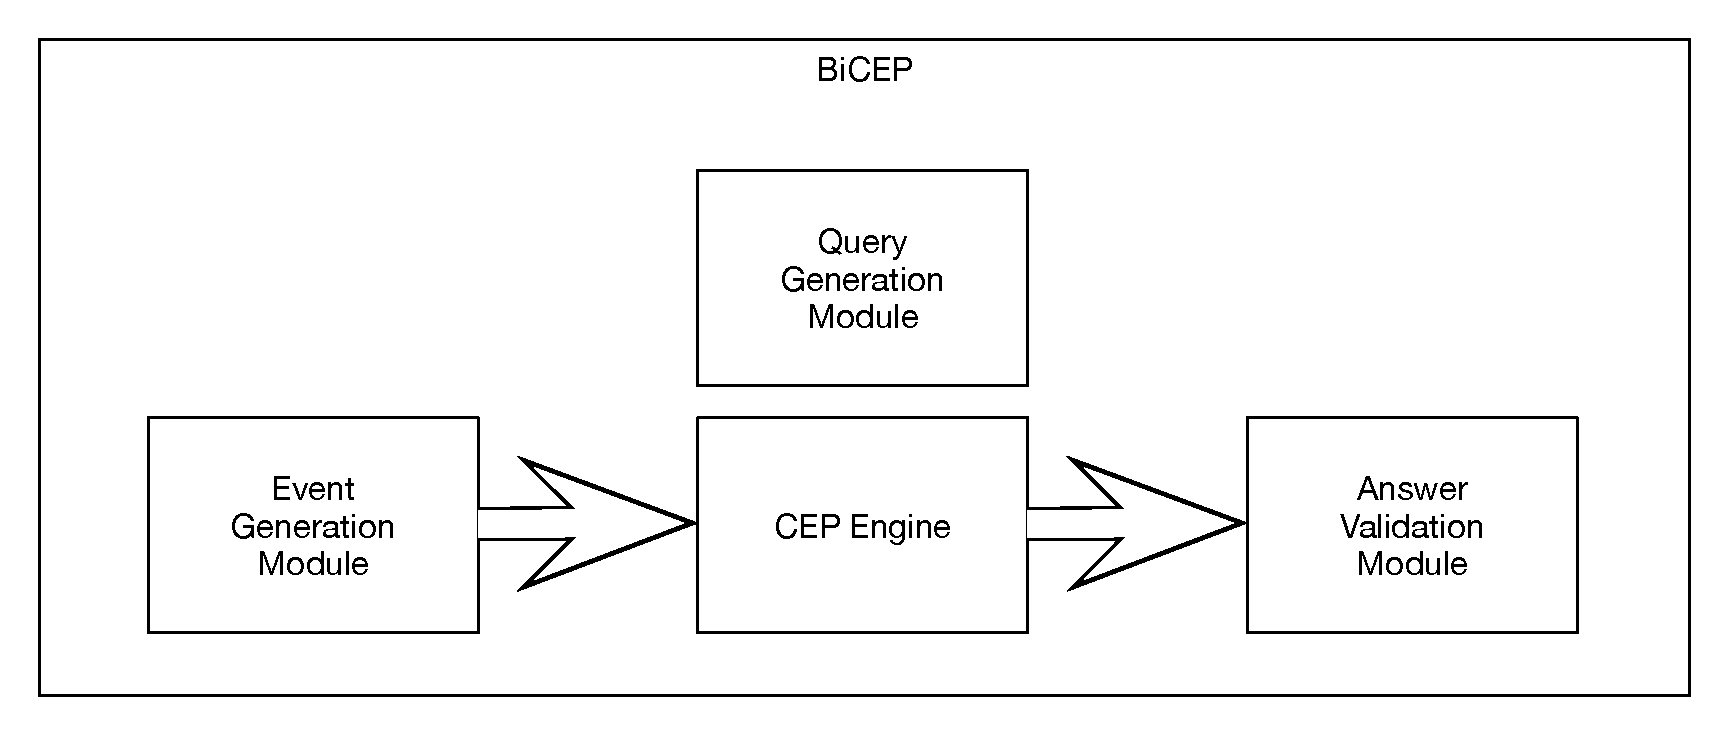
\includegraphics[width=\linewidth]{images/bicep_schema}
	\caption{BiCEP system  modules and the CEP engine} 
  	\label{fig:bicep-schema}
\end{figure}

BiCEP project also presents an first schema model for a benchmarking system, reported in Figure \ref{fig:bicep-schema}. The BiCEP benchmarking system will produce all the input trough the Event Generator Module, and consume the result output from the BiCEP CEP engine, with the Answer Validation Module. The Figure above also show how the CEP engine in interfaced with BiCEP modules, in order to ensure that any buffering, event cleaning or event transformation phase that happens at the CEP engine is part of the overall performance measure. Synthetic benchmarks offers many benefits like data availability, experimental control, and scalability. However, it is is hard to develop a synthetic benchmark that is representative of such a wide range of CEP applications and at the same time. BiCEP development is oriented towards a set of small domain specific synthetic benchmarks with different data sets and different queries \cite{bizarro:DSP:2007:1143}.

Finally, BiCEP project presents a set of metrics for CEP benchmarking, the most relevant ones in performance evaluation context are: \textit{Response time}: the time since the last event of some event pattern is fed into the system until the system notifies the event pattern detection. \textit{Scalability} in order to compare system with different scale levels; \textit{Adaptivity} the system response to input variation is mandatory, because CEP system rarely face stable input streams that allow the CEP engine to reach a steady state condition.



\subsection{Stream Reasoning Benchmark}
%\subsubsection{SRBench}
SRBench [5] proposes a suite of test queries and defines metrics to evaluate the
performance of the system. This benchmark contains 17 queries to gather the
properties of the RDF stream engines. The queries vary to ensure that several
features of the target system are tested: queries involving single or multiple input
streams, queries over stream-only data sources or over mixed stream and static
data source, etc. In [5] the authors applied the benchmark on the existent RDF
stream engines, and explained the differences in term of supported functionalities.
Time and memory performance tests, and scalability tests are not targeted
in the actual version of SRBench.
%\subsubsection{LSBench}
LSBench [6] proposes three tests to evaluate the RDF stream engines. The
first one is a functional test to verify the operators and the functionalities supported
by the engines: it is a test similar to the one proposed by SRBench. The
second test is a correctness test: its goal is to verify if the tested RDF stream
engine produces the correct output. Actually this analyses only the number of
produced answers, assuming that the contents of the output are correct. Finally,
the third test is a maximum input throughput test: it has the goal evaluate the
maximum throughput of the RDF stream engines. This test is done increasing
the rate of data in the stream and verifying the number of the answers. For each
test a set of 12 queries is provided; similarly to SRBench, the queries vary to
take into account different features of the engines (single and multiple streams,
presence of static data, etc)

%\subsubsection{Correttezza}
%\subsubsection{Seven Commandaments}



%--------------------------------------------------------------------------------
% problem settings
%--------------------------------------------------------------------------------
\chapter{Problem Settings}
\label{chap:problem-settings}
\chapter{Problem Settings}

In this chapter we present firstly the question that leads our research and the motivations which sustain it. Next we extend in Section x  the requirements posed by the research question and the issues it involves. In the end we provide the technical formalization of those requirements and why our work must cover them, which issue they solves and which limitation we have to face to.

\section{Overview}
Stream Reasoning research filed wonders to achieve a tight integration of known reasoning systems and DSMS, to exploit reasoning techniques upon rapid changing information \cite{Background SW, DSMS, SR}. An RDF Stream Processing Engine, shortly RSP Engine, is the abstraction that realizes this integration: it can  manage rapidly changing worlds at the semantic level and answer complex queries typical of Semantic Web. The Stream Reasoning community is working on the standardization of a protocol to talk with RSP Engines, which actually can be implemented applying a number of RSP techniques. Their number is increasing together with the need of shared practices and tools to perform analyses and evaluations. As stated in Chapter 2, benchmarking RSP Engines is possible thanks to the proposed RDF streams, continuous queries, and performance measurements. The critics on these works have showed their limits and further developments partially went beyond \cite{paper paper}. However, the the community still lacks the formalization of a comparative approach and an infrastructure that allows to apply it rigorously.

In this thesis we propose \namens, a framework that tries to solve the Stream Reasoning need of a Systematic Comparative Approach on RSP Engine evaluation.



\section{Requirements} \label{sec:requirements}

We developed \name in order to simplify and support Systematic Comparative Research Approach on RSP engines. To this extent we need to answer the following questions: 
\begin{enumerate}
\item[Q.1] How can the behaviour of system be evaluated? 
\item[Q.2] What makes this evaluation rigorous? 
\item[Q.3] How can this rigorous evaluation be automated?
\end{enumerate}

A proper answer to Question Q.1 can be stated exploiting the traditional definition of \textit{experiment}: a test under controlled conditions that is made to demonstrate a known truth or examine the validity of an hypothesis. Going deeply, we answer Q.2 bringing about the notions of \textit{reproducibility}, \textit{repeatability}, and \textit{comparability} of experiments. The concepts we identified make easy to answer Q.3 formalising the technical requirements for \namens.

Reproducibility is related to the variation in measurements made on a subject under changing conditions. The concept of experiment gather this conditions. \name must allow its users to define it in details: 
\begin{enumerate}
\item[R.1] it must be \textit{test data independent}, thus allowing users to chose relevant RDF data streams and ontologies from their domain of interest. %R.2.1
\item[R.2] it must be \textit{query independent}, thus allowing users to register relevant queries from their domains of interest. %R.2.2
\item[R.3] it must be \textit{engine independent}, thus allowing users to put an RSP engine on the test stand by the means of easy to implement software interfaces, e.g., it should adopt an event-base architecture as normally done by RSP engines and present events to RSP engine in a simple to parse RDF serialisation. %R4 e R5
\item[R.4] it must include a \textit{basic set of performance measurements} \cite{DBLP:conf/esws/ScharrenbachUMVB13} including \textbf{Latency} -- defined as the delay between the injection of an event in the RSP engine and its response to it --, \textbf{Memory Usage} -- defined as the difference between total system memory and free memory --, and \textbf{Completeness \& Soundness} of query-answering results.  %R2.3
\item[R.5] it should enable users to extend the test stand adding their own software sensors in order to other performance measurements %???
\end{enumerate}

In terms of software engineering the list of requirements above demands an \textit{Extendable Design} [R6], i.e.,  the possibility to replace theoretically each module with one with the same interfaces, but different behaviour, without affecting architecture stability.

Repeatability of measurements regards the variation in repeat measurements made on the same subject under identical conditions. \name must not affect the RSP engine evaluation to grant it. This from a practical point of view poses two requirements to the test stand:
\begin{enumerate}
\item[R.7] it must not be running when the RSP engine is under execution. %R.1.2
\item[R.8] it must have reduced (and possibly constant) memory footprint. %R.1.1
\end{enumerate}

The comparative research is case-oriented. It allows the systematic analysis of complex cases, exploiting comparable metrics. The complex cases are seen as configurations, a combination of known properties, upon which is possible to identify parallelism or state contrasts. A Systematic Comparative Research Approach (SCRA) requires firstly the definition of \textit{Metrics that allow comparison} and standardization of \textit{Evaluation conditions}.  \name must support the collection of the performance measurements as custom metrics [R.9]; again the concept of experiment is required a formalization for the execution setting. The next step consists in providing \textit{Tools for qualitative analysis}, which allow visualisation of the results [R.10].

Last but not least, to simplify SCRA is important to identify \textit{Simple terms of comparison}, which have an experimental validity. \name contains specific modules to fulfil this requests, more details about them in Chapter 6 . Those modules support the consequent need of \textit{Examples of successful analysis and evaluations}, which can be exploited as guidelines. Chapter 7 of this thesis present a set of experimental evaluations which show deeply the potential of \name.

%--------------------------------------------------------------------------------
% heaven
%--------------------------------------------------------------------------------

\chapter{Heaven - Design}
\label{chap:heaven}
In this chapter we present  \namens,  an open source framework for Systematic Comparative Research on RSP Engine.
It consists in four baselines and two main components: the Test Stand and the Analyser. Firstly, Section \ref{sec:teststand} introduces the Test Stand, which satisfies requirements from R.1 to R.8 and from R.10 to R.12, by executing experiments on an RSP Engine. Section \ref{sec:baselines} describes the Baselines, four RSP Engines that are included in \name as naive terms of comparison, since they fulfil requirements R.13 and R.14. Finally, Section \ref{sec:analyser} presents the Analyser, which addresses requirements R.9 and R.10  allowing the user to visualise, investigate and compare experiment results. %Soundness and completes of the query answering process are assessed post-hoc by comparing the results of an RSP engine with a term of comparison whose results are correct (see Section 5).

\section{Test Stand}\label{sec:teststand}

Aerospace engineering defines an Engine Test Stand as a facility used to develop, study and characterise engines. It allows to test operating regimes and offers measurement of several variables associated with engine process. A Test Stand may uses actuators for attaining a specific engine state, which is a unique combination of the engine properties. The information collected through the sensors depends on the engine manufacturer, which usually provides his own stand or the facilities to test the engine with commercial solutions. The Test Stand executes black box analysis, because usually the engines does not allow easily to interact with its internal mechanisms.

A Test Stand can be described similarly in the SR context. The definition above still holds its relevance with the difference that the tested engines are IO-Systems. An RSP Engine consumes an RDF Stream and  produces a new one, by applying queries under some entailment regime and w.r.t. an ontology which does not change over time. Describeing an RSP Engine means understanding the relation between input stream, the queries registered to it and what we call "operational semantics", which requires to know the RSP Engine internal process. Indeed, black box testing is the only possible one with a Test Stand, even having access to the entire RSP Engine code. Anyhow, \name Test Stand allows the user (the RSP Engine developer) to extend the sensors set add its own ones, according to requirements R.7 and R.10. In this way is possible to develop a specific testing procedure for a given engine.

\subsection{Architecture \& Workflow}\label{sec:arch-workflow}

\begin{figure}[tbh]
\centering
\includegraphics[scale=0.37]{images/schema2}
\caption{\name modules and workflow} 
\label{fig:architecture}
\end{figure}

\noindent An aerospace test stand exploits different modules to simulate the operating regime for the engine in use ( i.e a module for fuel distribution, one for the engine mechanic support or to enable users interaction during the execution ). \name \textsc{Test Stand}  is modular, it consists in stand-alone components that can be replaced with ones with the same interfaces [R.10]. At this moment, three modules compose the \textsc{Test Stand}:
\begin{itemize}
\item the \textsc{Streamer}, a source for the input RDF Stream
\item the RSP Engine we want to test;
\item the \textsc{Result Collector}, a data acquisition system for both the query results and the gathered measurements.
\end{itemize}
Figure \ref{fig:architecture} shows both the architecture of \name TS and its workflow.

We start presenting how the modules are configured: the components above are arranged into a pipeline and communicates exchanging events [R.11].  The execution starts with the \textsc{Streamer}, which hides the data generation logic in order to obtain data independence [R.1]. It pushes an RDF Stream directly to the mounted RSP Engine. It is up to the \textsc{Streamer} to respect [R.5] and not to influence the memory footprint with heavy data loading tasks. 

An interface adapts the event flow to the RSP Engine in use, fulfilling [R.2] (Engine Independence) and hiding the query registration process [R.3] (Query independence), which happens at engine level and is up to the RSP Engine provider.

The \textsc{Result Collector} is at the tail of the pipeline. It is part of the \textsc{Test Stand} because the performance measurements are processed and gathered during the execution, together with the queries results data.  The evaluation usually happens a-posteriori trough the Analyser (Section \ref{sec:analyser}). However, real time analysis of the performance measurements are possible, but they may violate some requirements like [R.4 and 5]. 

Last but not least, the Test Stand has an external structure that sustains other modules and can be considered as a module itself. It allows the user to control the process through accessible APIs and it adds the data gathered during the execution to the query results, controlling the process and ensuring that the \textsc{Test Stand} does not run when the RSP Engine run  as required by [R.4]. \\

\noindent The Test Stand accepts as input an \textsc{Experiment} in the form of a tuple $<\mathcal{E},\mathcal{D},\mathcal{T},\mathcal{Q},>$ where:
\begin{itemize}
\item $\mathcal{E}$ is the RSP Engine subject of the evaluation (satisfying requirement [R.3]); 
\item $\mathcal{D}$ is the input dataset [R.1]; 
\item $\mathcal{T}$ is the ontology [R.1]; 
\item $\mathcal{Q}$ is the query to be continuously answered by $\mathcal{E}$ [R.2]. 
\end{itemize}

Gathering different metrics is relevant from an experimental point of view: indeed, ask the system for the memory usage may influence the latency calculous or saving on disk the query results may influence the memory footprint. Indeed, we define there main kinds of experiment distinguishing on the data we want to sample and save.:
\begin{itemize}
\item Latency Experiment, where only the latency is calculated and no query result is saved on file
\item Memory Experiment, where only the memory is gathered and no query result is saved on file
\item Query Experiment, where query results are saved on file.
\item Any combination of the previous experiment types.
\end{itemize}

\noindent The Entity Relation diagram in figure \ref{fig:er} presents data model of the \textsc{Test Stand} . The diagram does not include entity attributes, but they are reported in the following Logic Schema:
\begin{figure}[tbh]
  \centering
	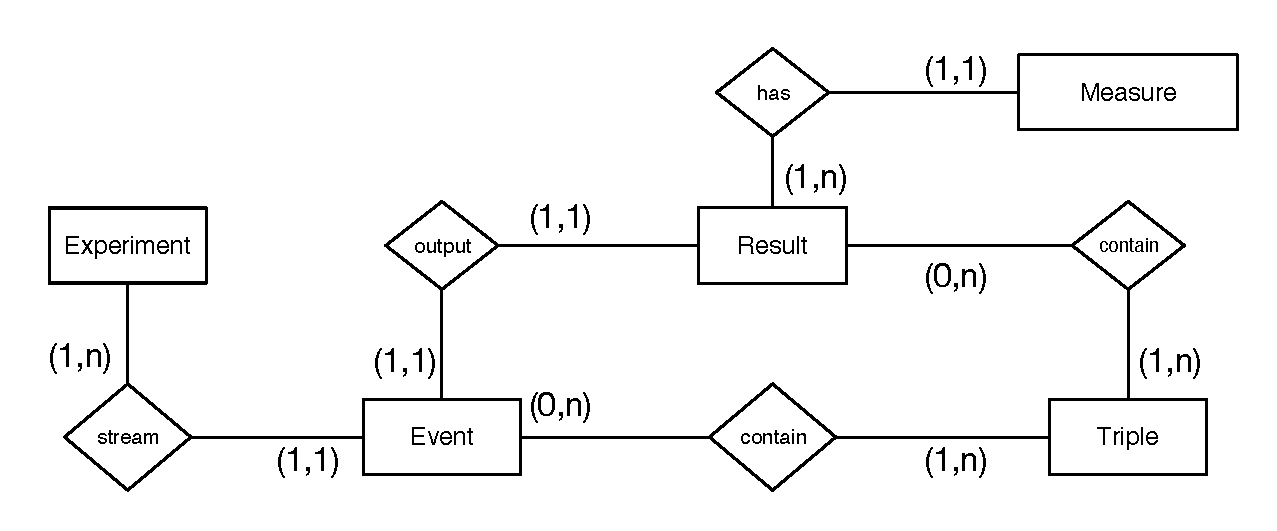
\includegraphics[width=\linewidth]{images/er-db}
	\caption{ER-Diagram For Experiment Output} 
  	\label{fig:er}
\end{figure}\\
\noindent\textsc{Experiment}(\underline{ID}, Timestamp Start, Timestamp End, Engine, Ontology, Query, Dataset, Description)\\
\textsc{Event}(\underline{ID, Experiment ID}, Timestamp)\\
\textsc{Result}(\underline{Result ID, Experiment ID}, Event ID)\\
\textsc{Measure}(\underline{ID}, Value)\\
\textsc{Measurement Set}(\underline{Measure ID, Result ID, Experiment ID})\\
\textsc{Triple}(\underline{S,P,O})\\
\textsc{Output Triple}(\underline{Result ID, Experiment ID, S, P, O})\\
\textsc{Input Triple}(\underline{Event ID, Experiment ID, S, P, O})\\

The \textsc{Experiment} entity contains all the metadata of the tuple $<\mathcal{E},\mathcal{D},\mathcal{T},\mathcal{Q},>$, which semantic is explained above. "Timestamp Start" and "Timestamp End" are relevant metrics for further analysis and system control. 
The \textsc{Event} is unique inside an \textsc{Experiment}, it is possible to send two events with the same timestamp and identical tripleset. The \textsc{Result}  is associated with one and only one \textsc{Event}. It contains the results to the engine queries w.r.t the active window and the set of the measure gathered during the execution. The \textsc{Measurement Set} table represent the relation between the \textsc{Result} and a number of measure that may variate  to fulfil requirement [R.7] (extendible measurement set). We include the concept of the \textsc{Triple} in order to model the content of \textsc{Event and Result}. \textsc{Input Triple} and \textsc{Output Triple} are the tables which represent the relation between \textsc{Triple} and respectively \textsc{Event} and \textsc{Result}
%a file, which contains a tuple with the sensor data and metadata for each event passed during the experiment execution; a set of TriG files that represents the window materialisation at each cycle, even in case of incremental reasoning. (It is also possible to save the non-materialised window, in order to verify the Completeness and Soundness of the reasoning procedure for the baselines).
%In practice the Test Stand outputs results in time series format and  the Analyser toolset has to handle this kind of information. 

\noindent The \textsc{Test Stand} orchestrates the communication between the upstanding models, forcing the \textsc{Streamer} to push events to the RSP Engine and the \textsc{Result Collector} to listen the output and collect the results.  To explain its workflow we split the process at the points when the modules exchange events. Indeed, each message represents a different logic step in the experiment execution cycle and we have distinguished six different ones.

In step (1) the \textsc{Test Stand} take the experiment and start the execution.  The \textsc{Test Stand} executes the experiment $<\mathcal{E},\mathcal{D},\mathcal{T},\mathcal{Q},>$ stressing $\mathcal{E}$ for a certain period of time looping through the steps from (2) to (5) illustrated in Figure \ref{fig:architecture}.                                                                                                                                                                                                                                                                                                                                                                                                                                                                                                                                                                                                                                                                                                                                                                                                                                                                                                                                                                                                                                                                                                                                                                                                                                                                                                                                                                                                                                                                                                                                                                                                                                                                                                                                                                                                                                                                                                                                                                                                                                                                                                                                                                                                                                                                                                                                                                                                                                                                                                                                                                                                                                                                                                                                                                                                                                                                                                                                                                                                                                                                                                                                                                                                                                                                                                                                                                                                                                                                                                                                                                                                                                                                                                                                                                                                                                                                                                                                                                                                                                                                                                                                                                                                                                                                                                                                                                                                      

In step (2), the \textsc{Streamer} pushes to $\mathcal{E}$ an event \textsc{CTEvent}. This event is a portion of an RDF Stream picked from the data $\mathcal{D}$ and it consists of a set of RDF triples with the same timestamp. In order to satisfy [R.12], it sends triple in N-Triple\footnote{\url{http://www.w3.org/2001/sw/RDFCore/ntriples/}}, which is the easiest RDF serialisation to parse.  

In step (3) $\mathcal{E}$ pushes to the \textsc{Result Collector} an event \textsc{OutCTEvent}. It contains the current answer to the query $\mathcal{Q}$ registered in $\mathcal{E}$ given the ontology $\mathcal{T}$. The \textsc{Test Stand} expects $\mathcal{E}$ to output result in N-Triple format. 

Notably, to place any RSP engine on the \textsc{Test Stand} (requirement [R.3]) \name provides a simple software wrapper that, when it receives a \textsc{CTEvent}, adapts it to the RSP engine specific format, pushes it in the RSP engine, and listens to the RSP engine output so to transform such an output in a \textsc{OutCTEvent}.

To measure performances (requirement [R.6]) the \textsc{Test Stand} performs several actions both before step (2) and after step (3) to collect data from the sensors. In step (4), those observations are added to the outputs of $\mathcal{E}$ as annotations and are pushed to the \textsc{Result Collector}.  We name \textsc{TSResult} the event that contains the sensor data plus the query results produced by the engine.  The \textsc{Test Stand} works in a single thread mode, blocking the execution of its components when it performs the measurements in (2) and (3) [R.4].  

Previous works about Stream reasoning \cite{} shows that the minimal performance measure set includes \textbf{Latency} -- defined as the delay between the injection of an event in the RSP engine and its response to it --, \textbf{Memory Load} -- defined as the difference between total system memory and the free one --, and \textbf{Completeness \& Soundness} of query-answering results. To measure latency, it starts a timer before (2) and stops it after (3). To measure memory load, it asks for the free memory of the system after step (3).

In step (5) the \textsc{Result Collector} saves \textsc{TSResult} for post process analysis [R.9], executed trough the \textsc{Analyzer}. It does so saving the content of any TSResult  [R.8].

\section{Baselines}
\label{sec:baselines}

\noindent In Chapter \ref{chap:problem-settings} we state that a Systematic Comparative Research Approach needs initial terms of comparison to lead the investigation. \name contains a set simple and easy-to-use RSP Engines called "baselines", developed to fulfil this lack . 
We exploit them to define some qualitative methods of investigation and to prove the usability of the Test Stand. 

In section \ref{sec:requirements} we identifies four characteristics that classify a case-study as a baseline inside a research field and here we report how \name Baselines are \textit{Elementary}, \textit{Relevant}, \textit{Simple} and \textit{Eligible}.

Early works on SR \cite{DBLP:conf/fis/ValleCBBC08,Walavalkar08streamingknowledge} describe the most simple approach to create a stream reasoning system: pipelining a DSMS with a reasoner. The DSMS is responsible to handle the data stream, moving from infinite sequences to finite (and processable) sets of events. The reasoner instead applies SPARQL queries on this set of events, exploiting its reasoning capabilities over a context that can be considered as static, but remains continuous.  As explained in Section \ref{sec:sfp}, we focus on this three the Stream Reasoning main building blocks: \begin{enumerate}
\item[1.] RDF streams;
\item[2.] An extensions of SPARQL to manage continuos data
\item[3.] reasoning algorithms
\end{enumerate}

\begin{figure}[tbh]
  \centering
	\includegraphics[width=\linewidth]{images/baselines-final}
	\caption{A: the architecture of the Naive baselines. B: the one of  the Incremental ones.} 
  	\label{fig:baselines}
\end{figure}
These there elements are summarised into RSP Engines, systems that can apply reasoning techniques upon rapidly changing information (Section \ref{sec:rspengine}). The approach above allow to develop an RSP Engine focusing only on link two existing technologies and develop the communication between them. But, how this design model fulfil the requirements poses in Section \ref{sec:requirements}?

Baselines \textit{Elementarity} is easy to be granted. The architecture above demands to choose a  DSMS which is a reliable solution in the CEP context  and the a general purpose rule engine which can be consider in the same way. We can consider this goal as reached when the couple elements are simple and valid terms of comparison w.r.t the state of the art.  Baselines \textit{Relevance} means to cover all the most important theoretical variants that the "pipeline approach" conveys. In terms of reasoning we can choose between to possible approaches and with reference to the data stream processing we have again two choice. Four baseline implementations cover these two main design decisions about the RDF Stream Model and the Reasoning procedures. 

The RDF Stream model describes how the input RDF Stream is processed, different systems accept data in different models, which depends on how RDF Stream is considered in terms of events contemporaneity. The two most relevant ones are:

\begin{itemize}	
\item Triple-based model, where the events pushed in the DSMS are timestamped triples. The timestamps are non decreasing, different triples could have the same timestamp to denote that they are contemporary.
\item RDF Graphs-based: the event pushed in the DSMS are timestamped RDF graph. The timestamps are increasing and the graph is used as a form of punctuation \cite{Tatbul2003b} to separate consequent portions of the RDF stream.
\end{itemize}

The Reasoning Architecture, the techniques to make inference, depends on the way data flow from the DSMS to the reasoner. Two reasoning solutions exist for the two triples data flow:

\begin{itemize}
\item Naive solution: (Figure \ref{fig:baselines}-A) the DSMS produces an RDF Snapshot of the current windows. Tt sends the entire content of the window to the reasoner, which materialises all the implied triples at each cycle. This is the approach implemented in the C-SPARQL Engine \cite{DBLP:journals/sigmod/BarbieriBCVG10} and in Sparkwave \cite{DBLP:conf/debs/KomazecCF12}.
\item Incremental solution (Figure \ref{fig:baselines}-B) the DSMS outputs the IRStream, the differences between the current window and the previous one. The $\Delta^{+}$ snapshot contains the triples that have just entered in the window, while the $\Delta^{-}$ snapshot contains the triples that have just exited from the window. The reasoner, using $\Delta^{+}$ and $\Delta^{-}$, incrementally maintains the materialisation over time. This approach is taken as term of comparison in \cite{DellAglio2014} and it is inspired from \cite{DBLP:conf/cikm/RenP11}.
\end{itemize}

Baseline \textsc{Eligibility} requires to check out all the performance measurements involved by the RSP Engine in use. We already stated that the choice of the DSMS and the reasoned may affect baseline \textsc{Elementarily}, but they also influence the performance of the engine. As reported in Section \ref{sec:teststand}, we take as initial measure set: Latency, Memory and of the query results Completeness and Soundness. The baselines must be at least comparable with commercial solutions in terms of degree of magnitude, in order to be Eligible for Latency and Memory. More consideration on this metrics are presented in Chapter of \ref{chap:evaluation}, which deeply answers the question with experimental results. On correctness of RDF stream processing \cite{DBLP:conf/semweb/DellAglioCBCV13} previous works explain the importance of external control on time to assure that the RSP Engine always outputs the correct answers (even when overloaded). The proposed baselines should take advantage of the ability of some DSMS to be temporally controlled by an external agent by sending time-keeping events to synchronise the internal time flow. %One time-keeping event is sent before injecting the triples in a \textsc{TCEvent} and another one after all triples in \textsc{TCEvent}  were sent. In this way all the triples in the TCEvent are consider contemporary by the 

Finally, baselines \textsc{Simplicity} comes from those parameters that directly influence the RSP Engine: the query $\mathcal{Q},$ and the entailment regime. $\mathcal{Q}$ should be eligible in terms of reasoning which means having an high materialisation effort of the implicit information entailed by the content of the window, given the ontology chosen by the user. The entailment regime should be a fragment of a language, maybe RDF-S,  which reduce complexity but preserves the normative semantics and the core functionalities. Moreover, what we state above about externally time control clarify the system workflow, so it is demanded to sustain baselines \textsc{Simplicity} too.

\section{Analyser}\label{sec:analyser}

The \textsc{Analyser} consists, from an engineering point of view, in one or more automated procedures which process the experiment results transforming raw data into an human-readable form. Actually, not all the analysing procedures can be completely automated and data analysis can not be always generalised. 

From a research point of view instead, the \textsc{Analyser} consists in a set of methods for data processing and analysing, which allow to refute or confirm hypothesis and improve existing models trough empirical findings.

In this Section we focus on the definition of the methods that compose the analysis, while in Section \ref{sec:analyser-impl} we detail much more which tools sustain the investigation at different levels, allowing data visualisation and deeper statistical investigations. \\

\begin{figure}[tbh]
  \centering
	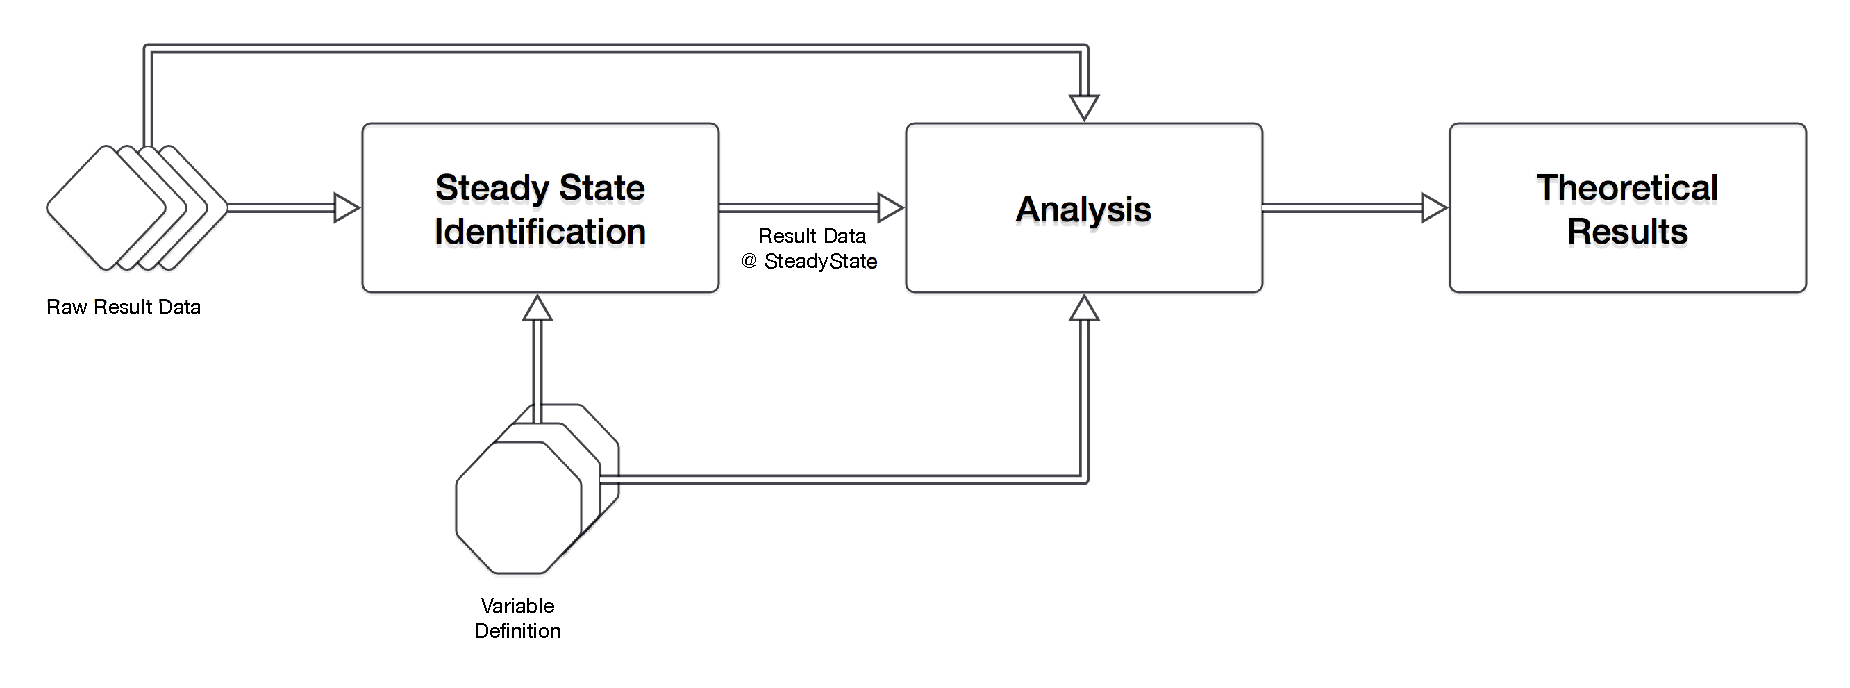
\includegraphics[width=\linewidth]{images/analyser-block-schema}
	\caption{From raw data processing to Theoretical results} 
  	\label{fig:analyser-block-schema}
\end{figure}

Figure \ref{fig:analyser-block-schema} shows the different phases of the data processing. The methods that compose the \textsc{Analyser} can be divided into three main steps, each one with different supporting tools and different goals.

\textsc{Analyser} takes as input the raw data produced by the \textsc{Test Stand} executing experiment, and the variable on which the analysis will be based on. In Section \ref{sec:teststand} we have described the \textsc{Test Stand} workflow. It outputs in times series form the data it gathers during the execution of an experiment. Which data the \textsc{Test Stand} gathers, the variable of the analysis, depend on the sensors it contains. To this extent the \textsc{Analyser} must parametric from the variable analysis. 

The First step in Figure \ref{fig:analyser-block-schema} is the \textit{Steady State Identification}, which can be seen as a pre-processing of the raw data.

\begin{figure}[tbh]
  \centering
	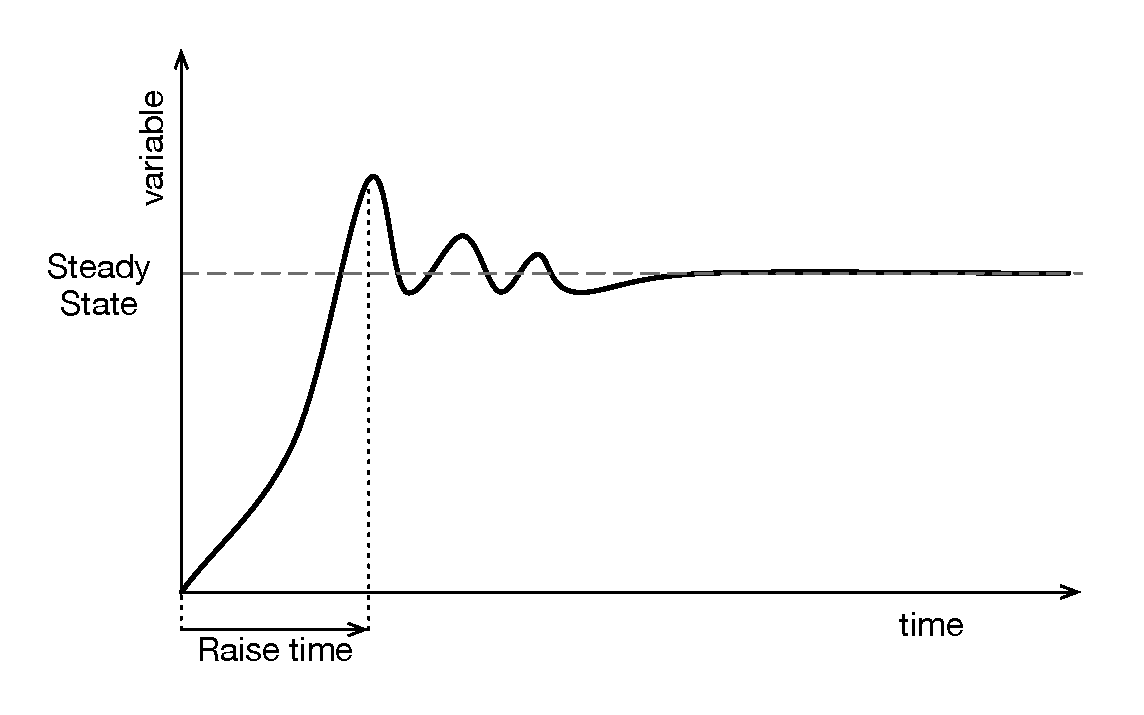
\includegraphics[width=0.5\linewidth]{images/steady-state}
	\caption{Time Series temporal domain} 	
  	\label{fig:steady-state}
\end{figure}

The Steady State is the moment when a dynamic system reaches the equilibrium for a certain variable. The identification of this condition is a common passage in almost any research on dynamic system and visual analysis can be exploited as the simplest tool to complete the task. Figure \ref{fig:steady-state} shows the typical behaviour in the time domain for a certain variable and also evidences the point when the the serie reaches the Steady State condition. Dynamic systems usually have an initial warm-up phase which negatively influences results and inhibit generalisation and comparisons. To properly contrasts results between $n$ different RSP Engines data must be standardized. In the \textit{Steady State Identification} step data are processed according to the variable definition, identifying which variable has reached a steady state condition. The Steady state identification process allow to understand the degree of reliability of the data, how we can assume a certain observation is confirmed and generalizable. 


Once the Steady State is identified is possible to proceed with data processing, which is summarised in Figure \ref{fig:analyser-block-schema} by the Analysis step. The analysis process all the data, but we distinguish the analysis w.r.t. the results form Steady State Identification step, because the analysis of the warm-up phase is a crucial part of the system comprehension and thus of the Hypothesis confirmation, as we will see in Chapter \ref{chap:evaluation}.


The last step in the high level Analyser process is consist in the formalisation of theoretical results. The aim of this step is obviously confirm or refute hypothesis formulated at experiment design level. However, \name has the aim of sustaining the empirical research which allow a new kind of observation that may improve existing theoretical model, changing the meaning of old hypothesis.

\subsection{Analysis Step}

The Analysis step we introduced above represents the concrete processing of the experiment result data. In this Section we detail this step. We decompose the analysis in four levels of different analysis details. We  introduce different analysis methods that each level involves. Figure \ref{fig:analysis-method} is a graphical representation of the Analysis stack, where the detail level grows from the top to the bottom. Further levels may be introduced at any point in the stack, since this design comes from the formalisation of our research work onver the Baselines presented in Chapter \ref{chap:evaluation}.

\pagebreak

Before presenting the stack level one by one, we introduce two concept about the experiment analysis:
\begin{itemize}
\item \textit{Intra Experiment Comparison} -  it means comparing results of different solutions (RSP Engine) within a single experiment, fixing only $\mathcal{D}, \mathcal{T} $ and $\mathcal{Q}$ or comparing different variables of the same solution  in a certain experiment.
\item \textit{Inter Experiment Comparison} -  it means comparing the same solution (RSP Engine) in different experiments or comparing how different solutions changes their behaviour in different experiments
\end{itemize}

\begin{figure}[tbh]
  \centering
	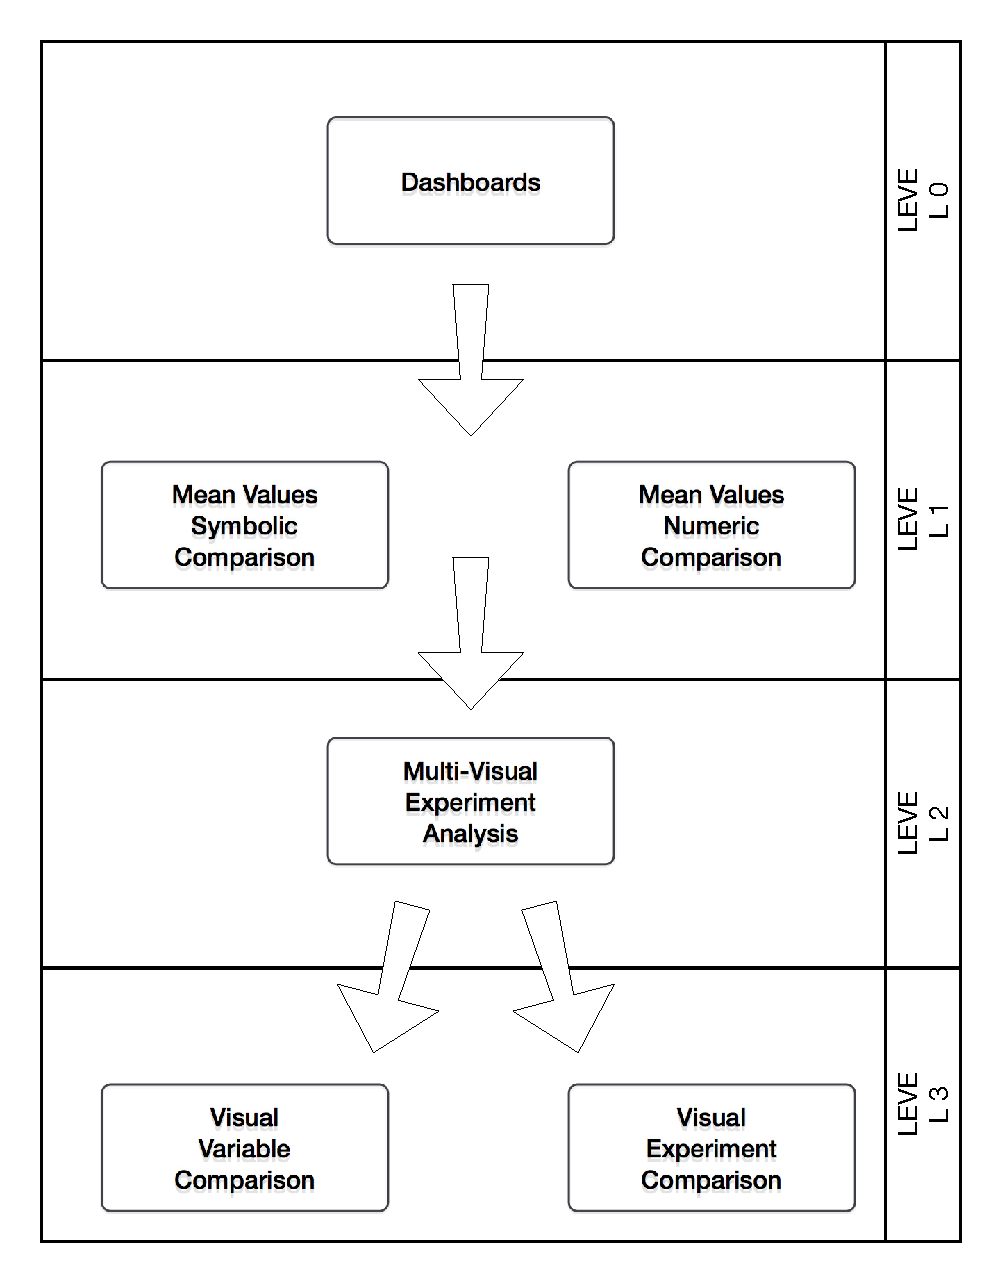
\includegraphics[width=\linewidth]{images/analysis-method}
	\caption{Analysis method stack. The level of analysis grows from the top to the bottom} 
  	\label{fig:analysis-method}
\end{figure}


\textsc{Level 0 - Dashboards}\\

Dashboards are the highest level of analysis offered by \namens. The Mean data value are presented in a n-dimension radar plot, which involves all the variables selected during the experiment design phase. Visual comparison of the data trough dashboards is natural when few variable are involved. It is easy to compare many solution and identify which one is the best, if any. Dashboard allow both inter-experiment comparison and intra-experiment comparison. 

The idea of a single visualisation method which allow to answer to any hypothesis is desirable, but not probable.  Unfortunately, the reliability of the methods depends on the system complexity and no only on the complexity of the method itself. Usually this level of analysis can not represent the entire system complexity. Moreover, if the Steady State condition is not reached by all the variable involved, the generalisation of any insight may be difficult. Further levels of analysis are required, at least for a better comprehension of those unpredictable results that refute even naive hypothesis, formulated on well known theoretical truths.

\textsc{Level 1 - Mean Value Comparison}\\

This Analysis level focuses on a single variable a time, exploiting both \textit{Intra-Experiment} and \textit{Inter-Experiment} comparison. Usually hypothesis verification requires the definition of multiple experiment, which variates for on or more parameters. This kind of analysis split  the dashboard representation, presenting one variable at time, comparing the results of different solutions.

Usually this comparison involves multiple experiment, presented in a easy-to-ready form, which evidence the differences between experiments.

\name makes possible two approach of this kind of analysis:
\begin{itemize}
\item \textit{Numeric} -  The comparison results are present in percentage form, quantifying how much a solution is better than another one, fixing some elements in the experiment.  With Numeric Mean variable comparison is possible to see how much, for a certain variable, the improvement of a given solution changes between experiment w.r.t. another one.

\item \textit{Symbolic} - it is a simplification of the Numeric Solution. Sometimes we only need no understand which solution is better, without focusing on numerical value. Symbolic solution required the definition of a tolerance threshold, for example 5\%, to distinguish when a solution is better, worst or equal to another one.

\end{itemize}
\textsc{Level 2 - Multi-Visual Experiment}\\


\textsc{Level 3 - Visual Comparison}\\
\begin{itemize}
\item \textit{Variable Comparison}
\item \textit{Experiment Comparison}
\end{itemize}








%--------------------------------------------------------------------------------
% conclusions and future works
%--------------------------------------------------------------------------------
\chapter{Conclusions and Future Works}
\label{chap:conclusions}
In this thesis work we have presented \name -- an open source framework for empirical evaluation of RSP Engines. \name aims enabling Systematic Comparative Approach in the Stream Reasoning research field trough an RSP Engine \textsc{Test Stand}, four Baselines of RSP Engines, and an \textsc{Analyser}. 

The motivations that led this work are included in Chapter \ref{chap:problem-settings}, while in Chapter \ref{chap:heaven} we described \name design and in Chapter \ref{chap:implementation-experience} we detailed the implementation of the \textsc{Test Stand}, the four Baselines and the investigation methods which compose the \textsc{Analyser}. Finally, we provided an empirical proof of \name potential in Chapter \ref{chap:evaluation}. Within the evaluation we compared the results of two experimental sets, SOAK and Stress tests, executed on the Baselines implementations. We learnt that, even when RSP Engines are extremely simple (e.g., the baselines), it is hard to demonstrate hypothesis formulated only from a theoretical knowledge. Thus empirical evaluation is required, because results emphasised the importance of conducting comparative research based on controlled experimental conditions and, thus, the need for a open source\footnote{\url{https://github.com/streamreasoning/HeavenTeststand}} framework like \namens.

The focus on the experimental infrastructure is the main difference between \name and previous work. While SRbench and LSbench focus on RDF streams and a suite of continuous SPARQL query, \name allows to compare RSP Engines based on any RDF stream, ontology, continuous query and entailment regime. It even enables to run experiments connecting to live data streams as those used in \cite{DBLP:conf/semweb/BalduiniVDTPC13}.	

In this chapter we recap this thesis works, presenting in Section \ref{sec:research-question-conclusion} our Research Question; in Section \ref{sec:research-results-conclusion} we briefly detail \namens, our work, which issues it involved and how we answer the research question. Finally, in Section \ref{sec:research-fw-conclusion} we point out \name limitations and future works of this thesis.

\section{Systematic Comparative Research Approach of RSP Engines}\label{sec:research-question-conclusion}

Stream Processing research field is growing and the number of techniques to semantically handle data stream is increasing. RDF Stream Processing Engines, a.k.a. RSP Engines, are systems able to answer continuous extensions of SPARQL queries over RDF Streams. Due to their complexity, a systematic comparison of such systems, under repeatable conditions, is hard. 

It is worth to note that, despite the Engineering epistemology of the Computer Science works, it is still present the lack of a Systematic Comparative Research Approach (SCRA) \cite{Tichy:1995:EEC:209090.209093}. SCRA is typical of those research areas which have to face very complex systems, and have difficulty to simplify the models. Architectural analysis are useful, but they are not sufficient to evaluate RSP Engine, because their behaviour must be studied during the execution. For this reason, the Stream Reasoning community has tried to define and develop solution to evaluates RSP Engines \cite{DBLP:conf/esws/ScharrenbachUMVB13}. Recent works like \cite{Zhang2012, LePhuoc2012c, DBLP:conf/semweb/DellAglioCBCV13} supported this approach with queries, dataset and methods. However the SR community still lacks an experimental infrastructure which enables the comparison of RSP Engines independently from RDF Stream, ontology, continuous query and entailment regime.  From aerospace engineering we borrow the idea of engine test stand: a facility to develop engine trough systematic testing under precise experimental conditions. Thus, we can formulate our research question as follow:\\

\textit{”Can an engine test stand, together with queries, datasets and methods, support Systematic Comparative Research Approach for Stream Reasoning?”}

%esperiment, reproducibility, repetability and comparability to enable the SRCA by a test stand
%simple terms of comparison to support the comparative research: SERE properties
%test stand design and implmentation fulfill the requirements posed
%Analyser consist in the definition of an analysis stack which extend% the traditonal top-down investiagtion based on hypothesis formulated on the model, trough empirical findings ad different level of analysis.
%We prove the value of the empirical resarch heaven test stand enables by evaluating the baselines
%we see that even for simple system like the baselines, which model is known, upredictable results may rise
%now it is possible to improve existing RSP engine model trough finding provide by the different analysi levels of the stack

In this thesis we answered such research question presenting \name, an open source framework for SCRA of RSP Engines. In the following we provides evidence of the positive results of our work, describing each phases it involves as how they are organised in this thesis.  

In Chapter \ref{chap:problem-settings} we describe how to borrow this idea of a test stand in the Stream Reasoning research field, with the goal of RSP Engine evaluation. We exploit the traditional experiment definition to grant the rigorous and systematic test of an RSP Engine. Three main experiment properties, \textit{reproducibility}, \textit{repeatability} and \textit{comparability}, allow us to formulate the requirements that a Test Stand for RSP Engine must fulfil, in order to answer our research question. SCRA, due to its case-oriented nature, demands simple terms of comparison, namely baselines, to exploit for initial evaluation examples. In Chapter \ref{chap:problem-settings} we detail which properties a baselines must have and we formulate them as  requirements for our work.

In Chapter \ref{chap:heaven} we describe \name design. We explain how the \textsc{Test Stand} and the Baselines should be to fulfil the requirements we posed. We introduce also the idea of the \textsc{Analyser} as an investigation stack, which extends the research of RSP Engine from the traditional hypothesis based approach to the empirical and comparative one. The higher levels of the investigation stack provide a statistical evaluation of experiment results, while the lower levels focus on RSP Engine dynamics offering an overview of the engine behaviour over all the experiment execution (further details of \name implementation and \textsc{Analyser} investigation stack can be found in Chapter \ref{chap:implementation-experience}).

%Our research question asks to demonstrate if a \textsc{Test Stand} for RSP Engine can support the SCRA for Stream Reasoning. 
In Chapter \ref{chap:evaluation} we show how the traditional top-down analysis are not enough for evaluating complex systems like RSP Engines, even in case of naive implementations. Our evaluation exploits an experimental set composed by SOAK Tests and Step Response Stress Tests, executed on the Baselines implementations that we included in \name framework. The results of the analysis show how the traditional research, which formulate hypothesis only on the RSP Engine model knowledge, is still meaningful, but it can be improved trough an infrastructure like \name \textsc{Test Stand}. The evaluation conducted in Chapter \ref{chap:evaluation} has shown that it is hard to demonstrate even naive hypothesis. RSP Engine dynamics can be only partially investigated from the statistical viewpoint We need further knowledge about the RSP Engine dynamics, which means observing their behaviour at once and over the entire execution of an experiment. In this way it is possible to apply SCRA at any details level it requires.\\

\noindent \name allows to drill down the analysis over an investigation stack which covers all the aspects of the dynamic system performance analysis. Previous works have defined how to evaluate RSP Engine systems \cite{DBLP:conf/esws/ScharrenbachUMVB13} and many attempts has been proposed \cite{Zhang2012, LePhuoc2012c, DBLP:conf/semweb/DellAglioCBCV13}. 

Thus, we can positively answer   our research question, stating that \name sustains SCRA and extends the traditional top-down analysis. The proposed queries and dataset can be evaluated systematically trough \namens, It is now possible to improve existing theoretical models trough the empirical findings \name points out, which were not easily available before.


\section{Limitations And Future Works}\label{sec:research-fw-conclusion}

During \name development we faced many issues related to the heterogeneous nature of RSP application domains. These concerns limit our work in different ways. They influence \name development in term of both design and implementation. Moreover, our research of RSP Engines  is actually restricted to \name Baselines within an extremely controlled experimental setting.

The limitations on \name design and its implementation must be faced improving its models and further developing the current implementation of the \textsc{Streamer}, \textsc{ResultCollector} and the \textsc{Test Stand External Structure}. On the other hand, the restrictions on the research of RSP Engine require to exploit \name \textsc{Test Stand} in order to pursue the analysis. Finally, we consider a further possible contribution the continuation of the research of the Baselines, which has its own scientific value, as Chapter \ref{chap:evaluation} partially evidenced.

Due to these limitations, the future works and possible extensions of \name belong to the following categories:
\begin{itemize}
\item \textit{Research of RSP Engine} - it involves the empirical evaluation of RSP Engine and the comparison of benchmarking results, which are our main research interests. Thus, we plan to support our research trough \namens.
\item \textit{Software Engineering and Development} - it involves future works focuses on the different aspects of \name software, which is extendible by design.
\item \textit{Research of Baselines} - it aims to provide a complete evaluation of the Baselines as simple terms of comparison for mature RSP Engines.
\end{itemize}

\noindent We aim extending the \textit{Research Work} creating a ready-to-use benchmarking suite built upon \namens, which allows to test any RSP Engine with a set of well defined experiments. Form preliminary studies we know that to cover the most important uses case an essential set of experiment must include the following tests:
\begin{itemize}
\item[T1] SOAK
\item[T2] Stress Step
\item[T3] Stress Sine Wave
\item[T4] Random Distribution (e.g., gaussian and exponential)
\end{itemize}

The experiments definition still follows the tuple $<\mathcal{E},\mathcal{D},\mathcal{T},\mathcal{Q}>$. The ready-to-use benchmarking suite will give the user the possibility to execute those test on his own RSP Engine. Moreover it should include \name Baselines as example of $\mathcal{E}$ and simple terms of comparison for benchmarking results.

SOAK Test [T1] and Stress Step Test [T2] are already part of this thesis work in a restricted form, while the other ones are not implemented yet. 

We develop [T1] and [T2] registering to our $\mathcal{E}$ as queries $\mathcal{Q}$ variations of the identity query, which a differ for window size $\omega$, because in the current stage of development it is possible to configure only the ontology and the entailment regime of the Baselines. We intend to continue the development of the Baselines, adding the possibility to register one or more continuous queries into them and exploiting more complex entailment regime than $\rho$DF. 

We have also to define which queries $\mathcal{Q}$ to include in all the experiments, considering many works in the field \cite{DBLP:conf/esws/ScharrenbachUMVB13, Zhang2012, LePhuoc2012c, DBLP:conf/semweb/DellAglioCBCV13}.

The current experiment sets [T1] and [T2] exploit LUBM ontology as $\mathcal{T}$ and the RDF Stream $\mathcal{D}$ is generated trough a module, the \textsc{RDF2RDFStream}, which adapts LUBM data to a streaming scenario (See Chapter \ref{chap:implementation-experience}). In order to generate data for all the remaining test sets [T3] and [T4] we have to extend the \textsc{RDF2RDFStream} to generate: a random flow with a given distribution (e.g., gaussian and exponential), and a sine wave flow (to mimic the periodic changes in the flow rates observed on social media streams \cite{DBLP:conf/semweb/BalduiniVDTPC13}).

Independently from the experiment set, we indent to extend the metrics gathered by \name \textsc{Test Stand}. Quoting from \cite{DBLP:conf/esws/ScharrenbachUMVB13} the possible extensions are:
\begin{itemize}
\item Response time over all queries (Average/$1^th$ Percentile/Maximum).
\item Maximum input throughput in terms of number of data element in the input stream consumed by the system per time unit.
\item Minimum time to accuracy and the minimum time to completion for all queries.
\end{itemize}

As we stated in Chapter \ref{chap:evaluation}, the content of the current window influences the RSP Engine performances for two factors: the window size before the reasoning and after. The second metrics is relevant for the RSP Engine evaluation. When the system has to handle a big number of outgoing triples we can observe a degradation in terms of memory and latency. Thus, an evaluation of the number of inferred triples w.r.t the window content at time $t$ allows to weight the engine performance results in relation to the input RDF Stream, helping to eliminate outliers and properly evaluate RSP Engines. Moreover, this observation opens new scenarios in the Stress Testing design, where the stress factor depends on the reasoning potential of the current window w.r.t a certain entailment regime.\\

\noindent Future works on \textit{Software Engineering and Development} regard the \textsc{Analyser}.  We aim to complete automate the analysis procedure, involving at least the current measurement set and tools. 

As a long term goal, we intend to standardise and publish the entire tool-set which supports analysis methods presented in Chapter \ref{chap:heaven}. We are imagining the \name \textsc{Analyser} as a Web-based environment where all existing RSP engines are already available and those: who want to run experiments, have just to configure them picking up one or more RDF streams, ontologies, and queries; who want to compare the results of its own RSP Engine can upload the raw data and wait for the evaluations results. A visual facility to compare different experiments and the publication of result experiments as linked data would complete this environment. \\


\noindent Finally, by evaluating the Baselines to prove \name potential we identified an intrinsic scientific value of this analysis. We would like to continue the \textit{Research of Baselines}, proving another contribution beyond the developments proposed above. In order to study the problem of responsiveness we have to add four alternative implementation of the Baselines, which do not exploit the external time control. The Baselines should be evaluated by [T1] T2] [T3] and [T4] but also with real data and a $\mathcal{T}$ different from LUBM, for example exploiting LS Bench queries and data to design an experiment set. 


%--------------------------------------------------------------------------------
% appendices
%--------------------------------------------------------------------------------
\part*{Appendices\label{part:app}\addcontentsline{toc}{part}{Appendices}}
\appendix
\chapter{\dots}
\label{app:one}
\input{content/app_one}

\chapter{\dots}
\label{app:two}
\input{content/app_two}

\bibliographystyle{plain}
\bibliography{tesi.bib}
\end{document}
